% Standalone graphical abstract (also embedded in the frontmatter of main.tex).
% Compile alone with: pdflatex graphical-abstract.tex
\documentclass[border=6pt]{standalone}
\usepackage{tikz}
\usetikzlibrary{positioning,arrows.meta,shapes.geometric,calc}
\definecolor{elsB1}{HTML}{08306B}
\definecolor{elsB2}{HTML}{2171B5}
\definecolor{elsB3}{HTML}{6BAED6}
\definecolor{elsB4}{HTML}{C6DBEF}
\definecolor{elsC1}{HTML}{66C2A5}
\definecolor{elsC2}{HTML}{FC8D62}
\begin{document}
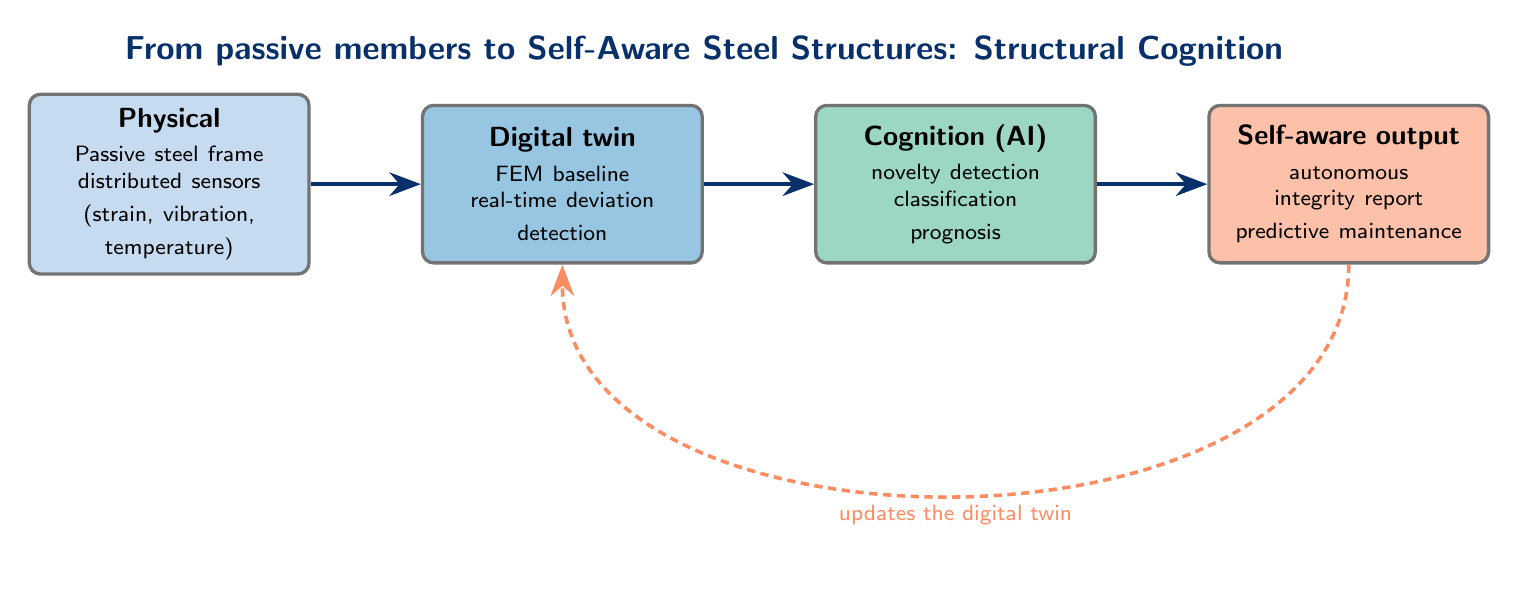
\begin{tikzpicture}[
  every node/.style={font=\sffamily},
  stage/.style={rectangle, rounded corners=4pt, draw=black!55, very thick,
                text width=3.2cm, minimum height=2.0cm, align=center, inner sep=5pt},
  arr/.style={-{Stealth[length=4mm]}, line width=1.3pt, elsB1}
]
  \node[stage, fill=elsB4] (phys)
        {\textbf{Physical}\\[3pt]\footnotesize Passive steel frame\\ distributed sensors\\ (strain, vibration, temperature)};
  \node[stage, fill=elsB3!70, right=1.4cm of phys] (twin)
        {\textbf{Digital twin}\\[3pt]\footnotesize FEM baseline\\ real-time deviation\\ detection};
  \node[stage, fill=elsC1!65, right=1.4cm of twin] (cog)
        {\textbf{Cognition (AI)}\\[3pt]\footnotesize novelty detection\\ classification\\ prognosis};
  \node[stage, fill=elsC2!55, right=1.4cm of cog] (out)
        {\textbf{Self-aware output}\\[3pt]\footnotesize autonomous\\ integrity report\\ predictive maintenance};
  \draw[arr] (phys) -- (twin);
  \draw[arr] (twin) -- (cog);
  \draw[arr] (cog) -- (out);
  \node[font=\sffamily\bfseries\large, elsB1, above=0.35cm of twin.north east, anchor=south]
        {From passive members to Self-Aware Steel Structures: Structural Cognition};
  \draw[-{Stealth[length=4mm]}, line width=1.3pt, densely dashed, elsC2]
        (out.south) to[out=270,in=270] node[below, font=\footnotesize\sffamily, elsC2]{updates the digital twin} (twin.south);
\end{tikzpicture}
\end{document}
